\documentclass[letterpaper, reqno,11pt]{article}
\usepackage[margin=1.0in]{geometry}
\usepackage{color,latexsym,amsmath,amssymb,graphicx, float}
\usepackage{hyperref}

\hypersetup{
colorlinks=true,
linkcolor=magenta,
filecolor=magenta,
urlcolor=cyan,
}

\graphicspath{ {images/} }

\newcommand{\RR}{\mathbb{R}}
\newcommand{\CC}{\mathbb{C}}
\newcommand{\ZZ}{\mathbb{Z}}
\newcommand{\QQ}{\mathbb{Q}}
\newcommand{\NN}{\mathbb{N}}
\newcommand{\st}{\text{ s.t.}\ }
\newcommand{\tn}[1]{\textnormal{#1}}
\newcommand{\m}{\textnormal{ m}}
\newcommand{\s}{\textnormal{ s}}
\newcommand{\K}{\textnormal{ K}}
\newcommand{\h}{\textnormal{ h}}
\newcommand{\W}{\textnormal{ W}}
\newcommand{\J}{\textnormal{ J}}
\newcommand{\Pa}{\textnormal{ Pa}}
\newcommand{\mol}{\textnormal{ mol}}
\newcommand{\Hz}{\textnormal{ Hz}}
\newcommand{\kg}{\textnormal{ kg}}
\newcommand{\cm}{\textnormal{ cm}}
\newcommand{\mm}{\textnormal{ mm}}
\newcommand{\N}{\textnormal{ N}}

\begin{document}
\pagenumbering{arabic}
\title{ELEC 221 Homework 3}
\date{October 27, 2021}
\author{Xander Naumenko}
\maketitle

{\noindent\bf Question 2a.} This system is linear, time invariant and causal. For linear, we see that when $x_1[n]=\alpha x_2[n]+\beta x_3[n]$ the output is

$$
    y_1[n] = \sum_{k=0}^{\infty} \alpha x_2[n]+\beta x_3[n]=\alpha\sum_{k=0}^\infty x_2[n]+\beta\sum_{k=0}^\infty x_3[n]=\alpha y_2[n]+\beta y_3[n]
$$

For time invariance we have 

$$
    T(x[n-n_0]) = \sum_{k=0}^\infty x[n-n_0-k]=y[n-n_0]
$$

Therefore it follows that $y$ is time invariant. Finally for causal, we have that 

$$
    h[n] = T\{\delta[n]\}=\sum_{k=0}^\infty \delta[n-k]=\begin{cases}
        0&\text{ for }n<0\\
        1&\text{ for }n \geq 0
    \end{cases}
$$

Since the impulse response is zero for negative $n$ the system is causal. 

{\noindent\bf Question 2b.} The system is not linear, since in general

$$
    T\{\alpha x_1[n] + \beta x_2[n]\} = |\alpha x_1[n] + \beta x_2[n]|\neq \alpha |x_1[n]| + \beta |x_2[n]|=\alpha y_1[n]+\beta y_2[n]
$$

Note that of course for specific inputs the equality above could hold, but in general it does not. The system is time invariant since $y[n-n_0]=|x[n-n_0]|=T\{x[n-n_0]\}$. The system is also causal, since it has the same impulse response as $y[n] = x[n]$ of $h[n]=\delta[n]$ which is obviously causal. 

{\noindent\bf Question 2c.} The system is linear, since 

$$
    T\{\alpha x_1[n] + \beta x_2[n]\}=(\alpha x_1[n] + \beta x_2[n])\cos(0.2\pi n)=\alpha x_1[n]\cos(0.2\pi n) + \beta x_2[n]\cos(0.2\pi n)
$$

$$
    =\alpha y_1[n] + \beta y_2[n]
$$

It is not time invariant, since 

$$
    T\{x[n-n_0]\}=x[n-n_0]\cos(0.2\pi n)\neq x[n-n_0]\cos(0.2\pi(n-n_0))=y[n-n_0]
$$

Note that again this inequality could hold for specific $n_0$, but is not true for all $n_0$. Finally the system is also causal since the impulse response is $h[n]=\delta[n]$ which is means it is causal. 

{\noindent\bf Question 2d.} Despite its appearences $y$ is not linear, since 

$$
    T\{\alpha x_1[n] + \beta x_2[n]\}=A\alpha x_1[n] + A\beta x_2[n]+2B
$$

which is not linear. It is time invariant, since 

$$
    T\{x[n-n_0]\}=Ax[n-n_0]+B=y[n-n_0]
$$

Finally it is not causal since the impulse response is $h[n]=A\delta[n]+B$ which is not zero for $n<0$. 

{\noindent\bf Question 2e.} See graph in Figure \ref{fig:2e}. 


\begin{figure}[htbp]
\centering
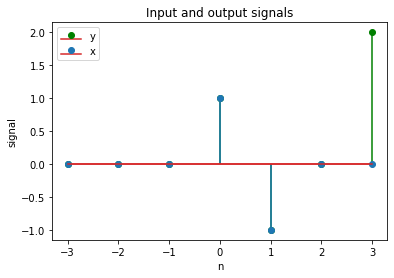
\includegraphics[width=\textwidth]{2e}
\caption{Graph for question 2e. Note that the first two points are overlapping}
\label{fig:2e}
\end{figure}

{\noindent\bf Question 2f.} Expanding it is true that $\tilde x[n] = 7x[n]+7x[n-1]$. Using the linearity property of the system we have that 

$$
    T\{\tilde x[n]\}=T\{7x[n]-7x[n-1]\}=7\delta[n]-7\delta[n-2]+14\delta[n-3]+14\delta[n-4]
$$

The graph of this output can be seen in figure \ref{fig:2f}. 

\begin{figure}[htbp]
\centering
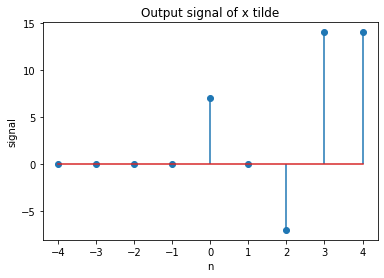
\includegraphics[width=\textwidth]{2f}
\caption{Output for question 2f}
\label{fig:2f}
\end{figure}

{\noindent\bf Question 3a.} To show it is necessary is to show the other direction of proof, i.e. the system is stable implies that $h$ is absolutely summable. To show this we will use the contrapositive, i.e. if $h$ is not absolutely summable then the system is not stable. Let $h$ be such that 

$$
    \sum_n\in\ZZ|h[n]|=\infty
$$

Next define $x$ such that 

$$
    x[n]=\begin{cases}1&\text{ if }h[-n]>0\\-1&\text{ if } h[-n] \leq 0\end{cases}
$$

Note that due to the way we define $x$, $h[n]x[-n]=|h[n]|\forall n\in\ZZ$. Then we get 

$$
    y[n]=\sum_{k\in\ZZ} h[k]x[n-k]
$$

$$
    y[0]=\sum_{k\in\ZZ}h[k]x[-k]=\sum_{k\in\ZZ}|h[k]|=\infty
$$

Thus $y[0]$ is unbounded. By the contrapositive this means the original statement was true. 

{\noindent\bf Question 3b.} The sufficient condition is that the input response sums to less than or equal to 1, i.e.

$$
    \sum_{n\in\ZZ} |h[n]|\leq1
$$

To show this assume that the input response is absolutely summable, then we have 

$$
    |y[n]|=\bigg|\sum_{k\in\ZZ} x[n-k]h[k]\bigg|\leq \sum_{k\in\ZZ}|x[n-k]||h[k]|\leq \max_{n\in\ZZ}|x[n]|\sum_{k\in\ZZ}|h[k]|=\max_{n\in\ZZ}|x[n]|
$$

Since this holds for all $y$, we can take the maximum to get 

$$
    \max_{n\in\ZZ}|y[n]|\leq\max_{n\in\ZZ}|x[n]|
$$

{\noindent\bf Question 3c.} To show it is necessary we must show that if the system is stable, then impulse response absolutely sum to less than or equal to 1. We will show the contrapositive, that if $\sum_{n\in\ZZ} h[n]>1$ then the system doesn't fulfill the inequality. To do this define $x$ as 

$$
    x[n] = \begin{cases}1&\text{ if }h[-n]>0\\-1&\text{ if } h[-n] \leq 0\end{cases}
$$

Similar to part a this gives that $x[-n]h[n]=|h[n]|$. Thus we have 

$$
    y[0]\sum_{n\in\ZZ}=\sum_{k\in\ZZ}x[-k]h[k]=\sum_{k\in\ZZ}|h[k]|>1=\max_{n\in\ZZ}|x[n]|
$$

Since we proved the contrapositive the original statement must be true. 

{\noindent\bf Question 3d.} Expanding, we get 

$$
    |H(e^{j\omega})|=\bigg|\sum_{k\in\ZZ}h[k]e^{-j\omega k}\bigg|\leq \sum_{k\in\ZZ}|h[k]||e^{j\omega k}|=\sum_{k\in\ZZ}|h[k]|
$$

For $H(e^{j\omega})$ to exist then it needs to be that the impulse response is absolutely summable. This is the exact same requirement that is both sufficient and necessary for an LTI system to be stable, so the frequency response exists provided the system is stable. 

{\noindent\bf Question 4a.} Writing out the definition: 

$$
    H_1(e^{j\omega})=\sum_{k\in\ZZ}h[k]e^{j\omega_0 k}e^{-j\omega k}
$$

$$
    H_1(e^{j\omega})=\sum_{k\in\ZZ}h[k]e^{-j(\omega-\omega_0) k}=H(e^{j(w-\omega_0)})
$$

{\noindent\bf Question 4b.} We know $(-1)^n=e^{j\pi n}$. Thus using part a we get that $H_2(e^{j\omega}) = H(e^{j(\omega-\pi)})$. This means that the passband is shifted by $\pi$, so $\omega_c\in(\pi, 2\pi)$. 

{\noindent\bf Question 4c.} Using properties of the conjugate, we get 

$$
    H^*(e^{-j\omega})=\sum_{k\in\ZZ}h[k](e^{j\omega k})^*=\sum_{k\in\ZZ}h[k]e^{-j\omega k}=H(e^{j\omega})
$$

{\noindent\bf Question 4d.} Expanding our definition for $H$: 

$$
    H_d(e^{j\omega})=\sum_{k\in\ZZ}h_d[k]e^{-j\omega k}=j\frac{dH(e^{j\omega})}{d\omega}=\sum_{k\in\ZZ}k h[k]e^{-j\omega k}
$$

Equating each part of the sum term by term (this is allowed because the relationship must hold for all $\omega$ and each of the $e$ terms are linearly independent), we find that $h_d[n]=nh[n]$ as desired. 

{\noindent\bf Question 4e.} We will gobackwards from the product of the frequency responses. Expanding: 

$$
    H_1(e^{j\omega})H_2(e^{j\omega}) = \sum_{k\in\ZZ}h_1[k]e^{-j\omega k}\sum_{n\in\ZZ}h_1[n]e^{-j\omega n}
$$

The product of the sums encompasses all possible combinations of $n$ and $k$, so this is equivalent to 

$$
    \sum_{k\in\ZZ}\sum_{n\in\ZZ}h_1[k]h_2[n]e^{-j\omega k}e^{-j\omega n}
$$

Since the sums are going over all integers we can offset either $n$ or $k$ while summing while maintaining equality, so 

$$
    =\sum_{k\in\ZZ}\sum_{n\in\ZZ}h_1[k]h_2[n-k]e^{-j\omega k}e^{-j\omega (n-k)}
$$

$$
    =\sum_{n\in\ZZ}\sum_{k\in\ZZ}h_1[k]h_2[n-k]e^{-j\omega n}
$$

$$
    =\sum_{n\in\ZZ}(h_1[n]*h_2[n])e^{-j\omega n}
$$

Letting $x[n]=\delta[n]$, we have that $T_1\{T_2\{\delta[n]\}\}=T_1\{h_2[n]\}=h_1[n]*h_2[n]=h[n]$. Thus the previous line simplifies to 

$$
    =\sum_{n\in\ZZ} h[n]e^{-j\omega n}=H(e^{j\omega})
$$

{\noindent\bf Question 4f.} For the first $h$: 

$$
    H(e^{j\omega}) = \sum_{k\in\RR} h[k] e^{-j\omega k}=\sum_{k\in\RR}(\frac14)^k v[k]e^{-j\omega k}=\sum_{k\geq0} (\frac{e^{-j\omega}}{4})^{k}
$$

This is a geometric series, so

$$
    =\frac1{1-(\frac{e^{-j\omega}}4)}
$$

For the second: 

$$
    H(e^{j\omega}) = \sum_{k\in\RR}h[k]e^{j\omega k}=1+e^{-j\omega}+e^{-j\omega 2}+e^{-j\omega 3}+e^{-j\omega 4}
$$

Finally for the third, I assume it was a typo and it was supposed to be a $v$ instead of $u$. If this is the case then the frequency response is 

$$
    H(e^{j\omega}) = \sum_{k\in\RR} h[k] e^{-j\omega k}=\sum_{k\in\RR}(\frac14)^k v[k+2]e^{-j\omega k}=\sum_{k\geq-2} (\frac{e^{-j\omega}}{4})^{k}
$$

This is the exact same as the the first part except offset by two, so applying the same principle, 

$$
    =e^{2j\omega} + e^{j\omega}+\frac1{1-(\frac{e^{-j\omega}}4)}
$$


\end{document}